\newpage
\section{Cross-talk in data}
\label{appendix:crosstalkData}

The effect of the $\Hbb$ tagger veto on the $\Hww$ tagged dijet
mass distribution
background (data) is shown in Figures~\ref{fig:HbbRatio}.
%The fraction of $\Hww$ tags which are also $\Hbb$ tags are small,


%\begin{figure}[htb]
\begin{figure}[ht]
\begin{center}
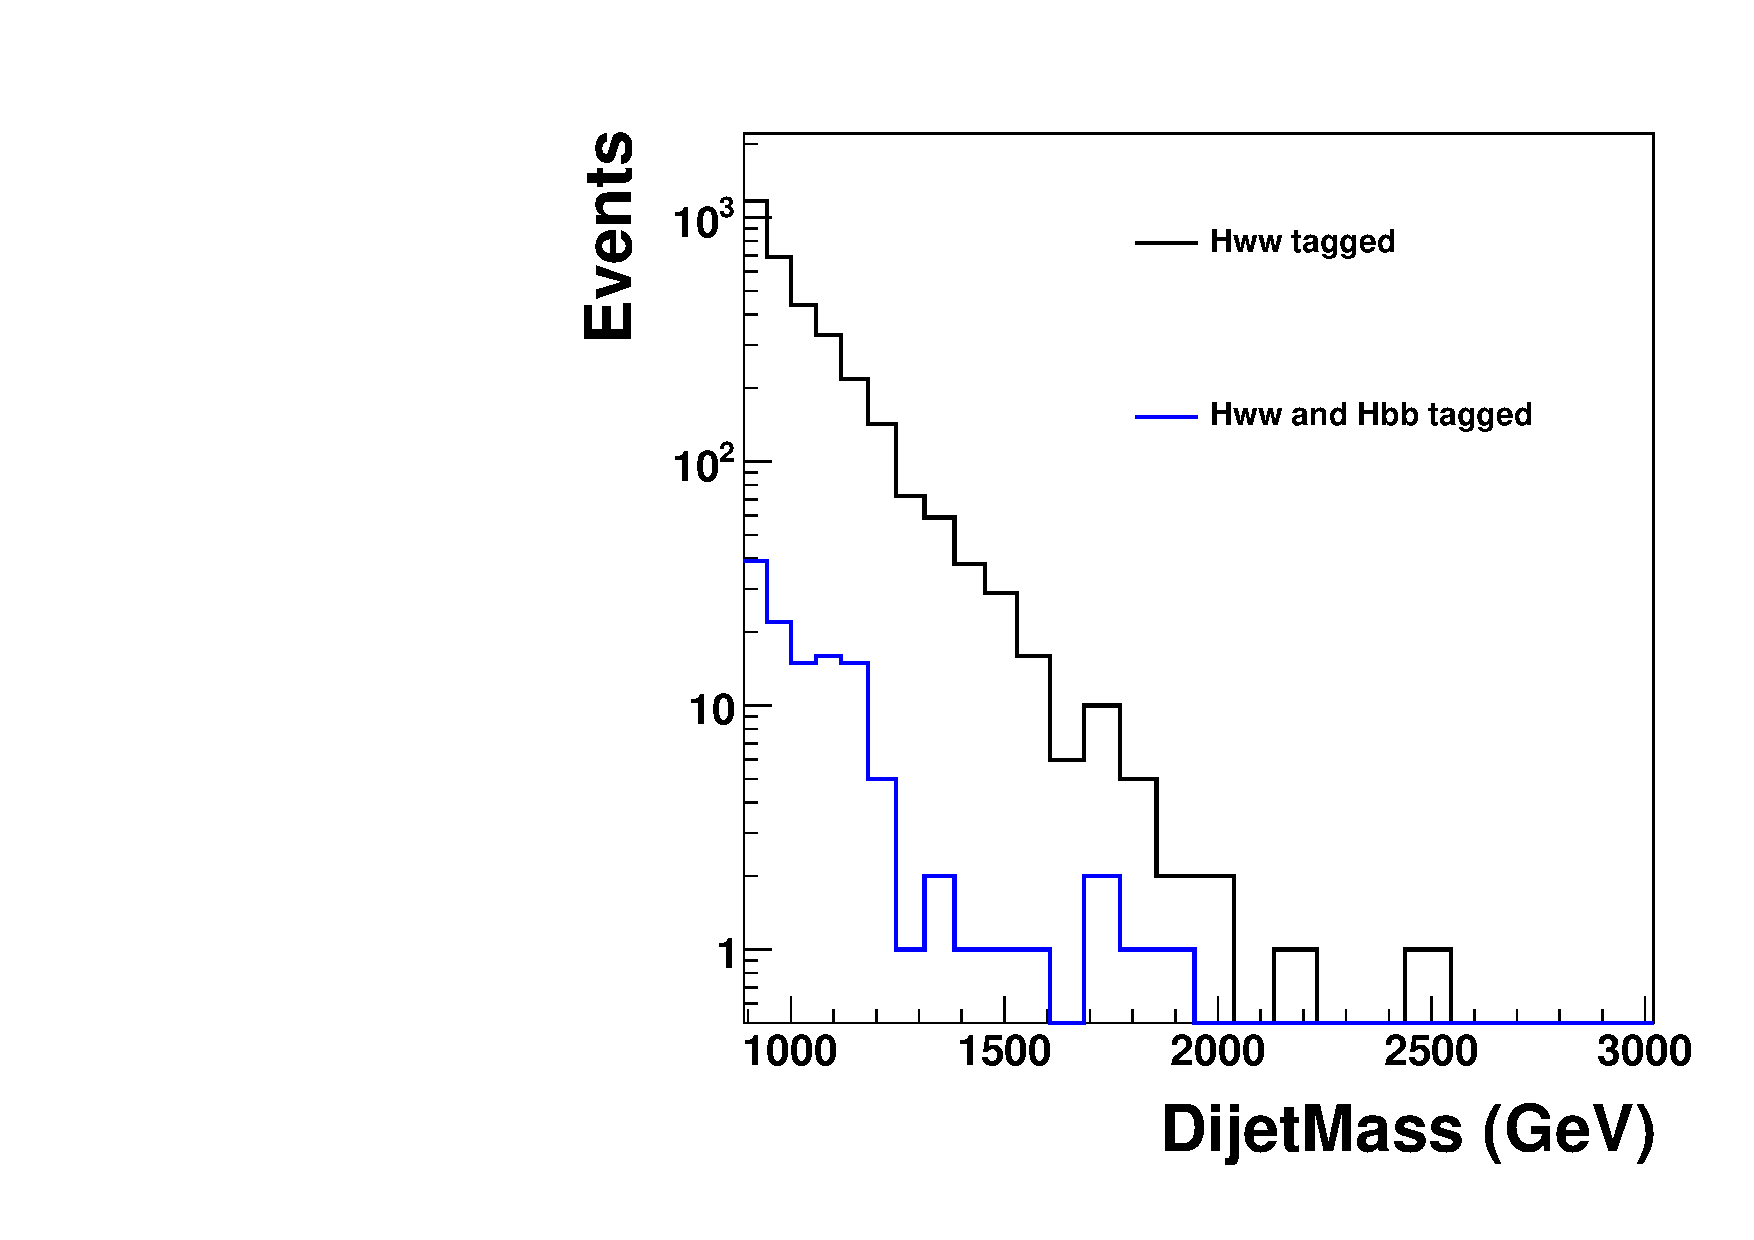
\includegraphics[width=0.49\textwidth, height=0.45\textwidth]{HqqqqZqqfigs/HbbHww/HighPurity.pdf}
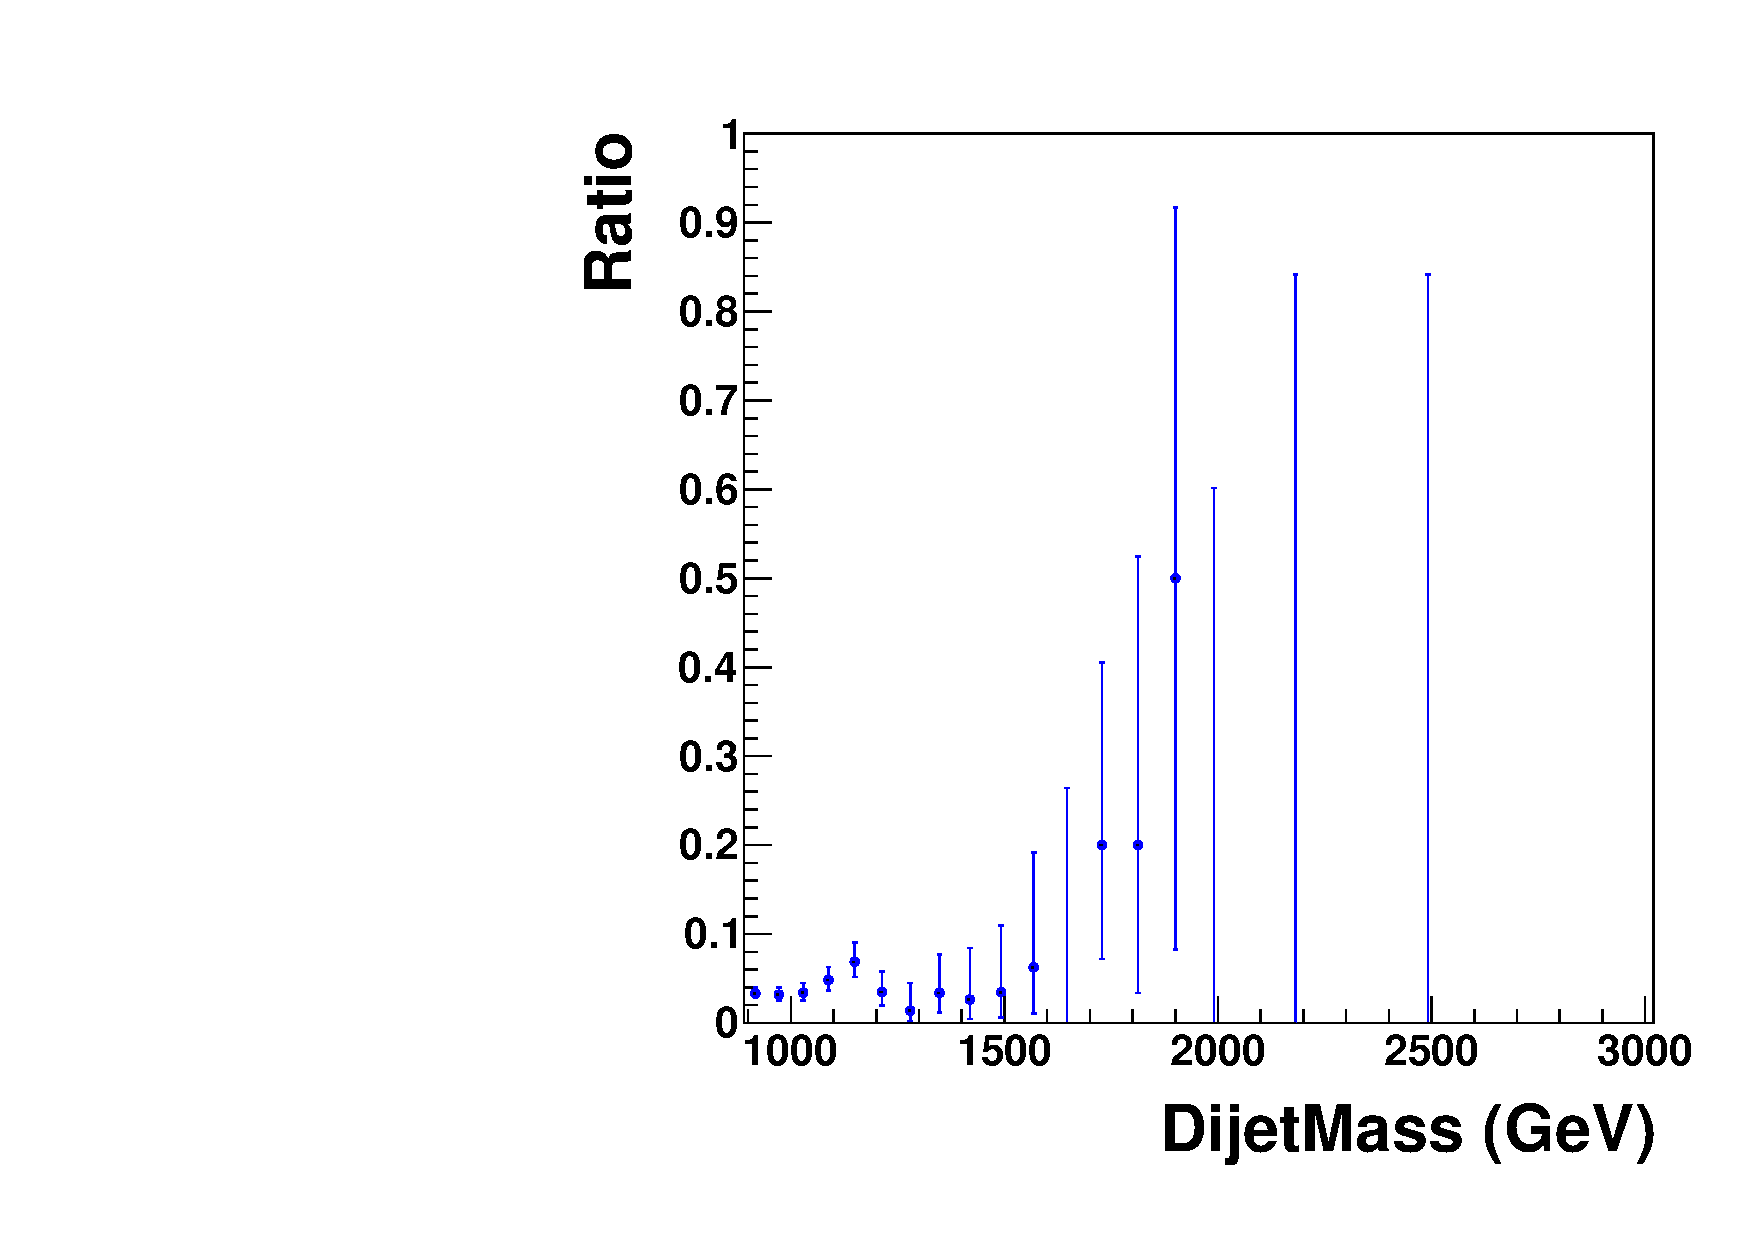
\includegraphics[width=0.49\textwidth, height=0.45\textwidth]{HqqqqZqqfigs/HbbHww/HighPurityRatio.pdf}
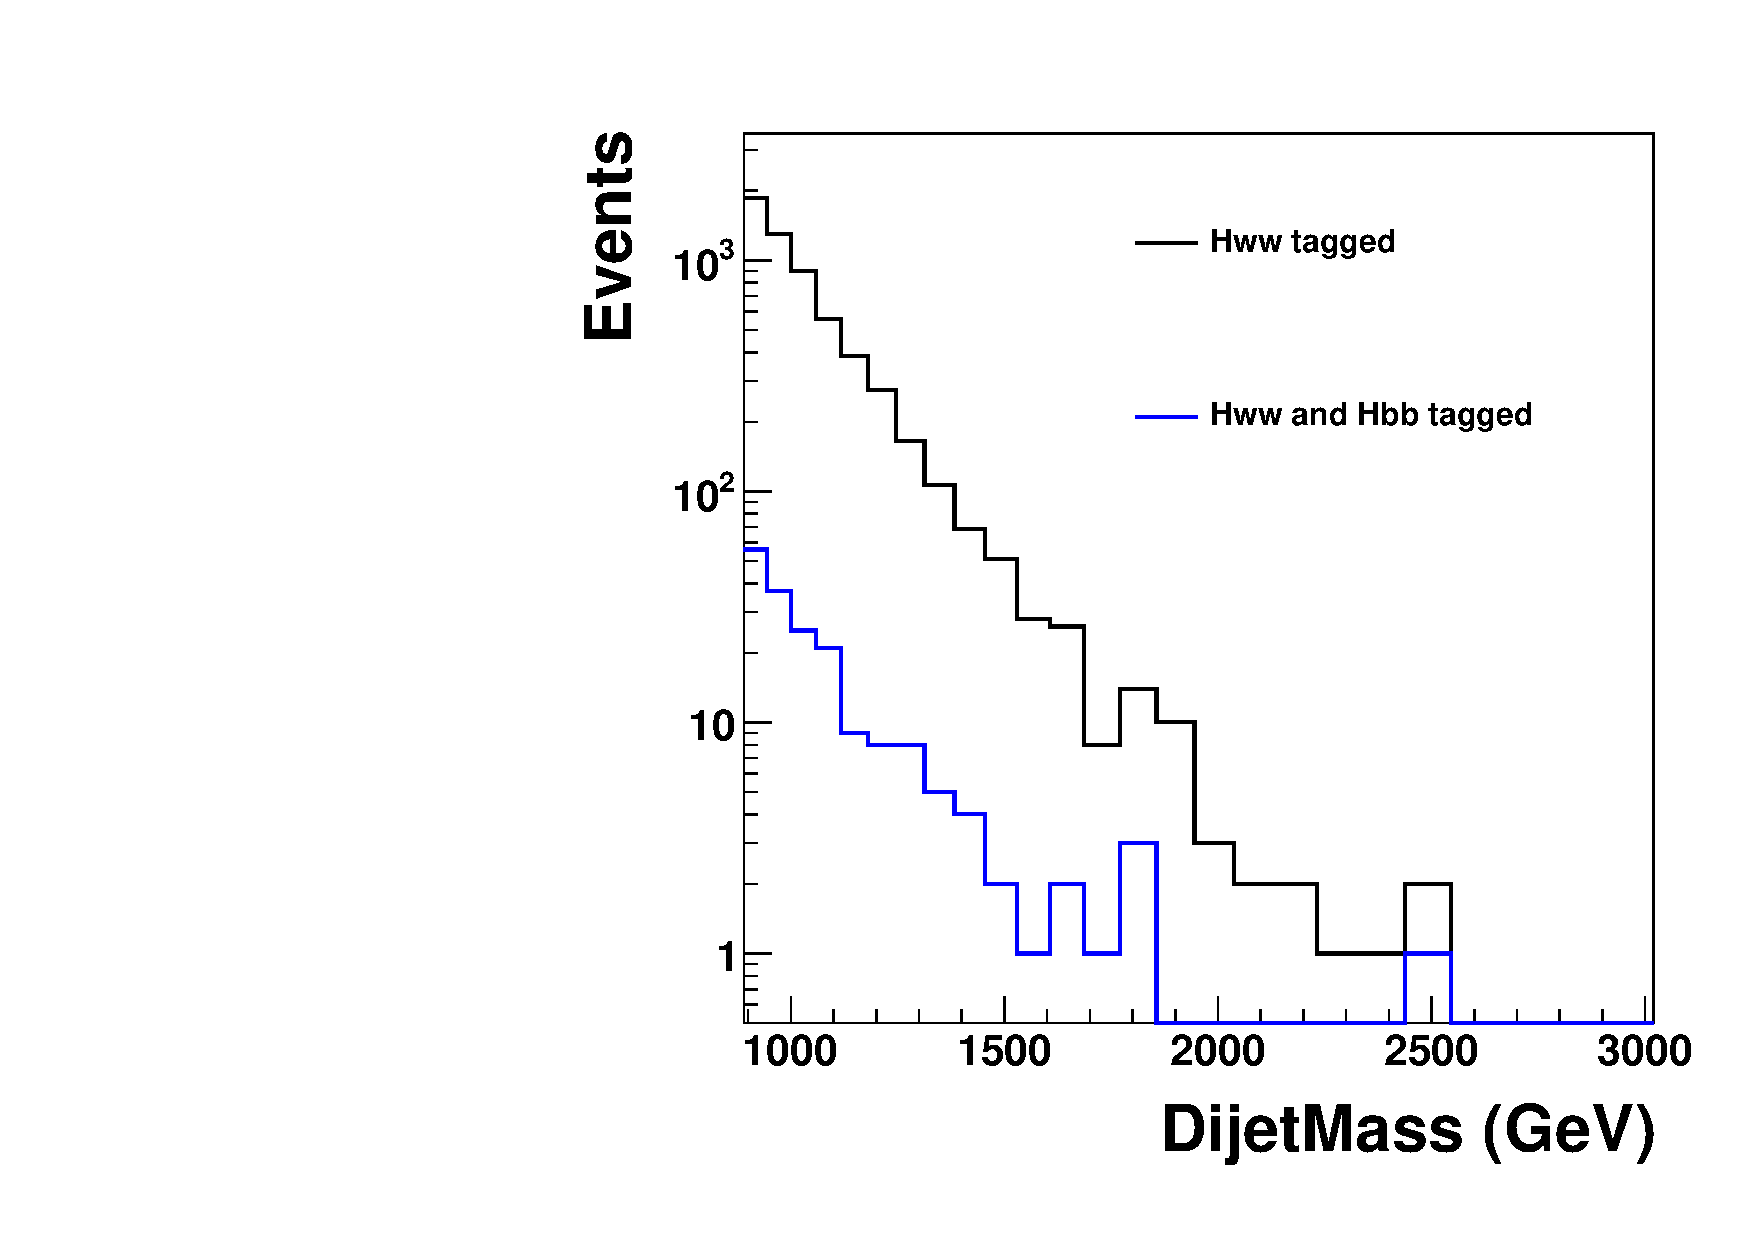
\includegraphics[width=0.49\textwidth, height=0.45\textwidth]{HqqqqZqqfigs/HbbHww/LowHPurity.pdf}
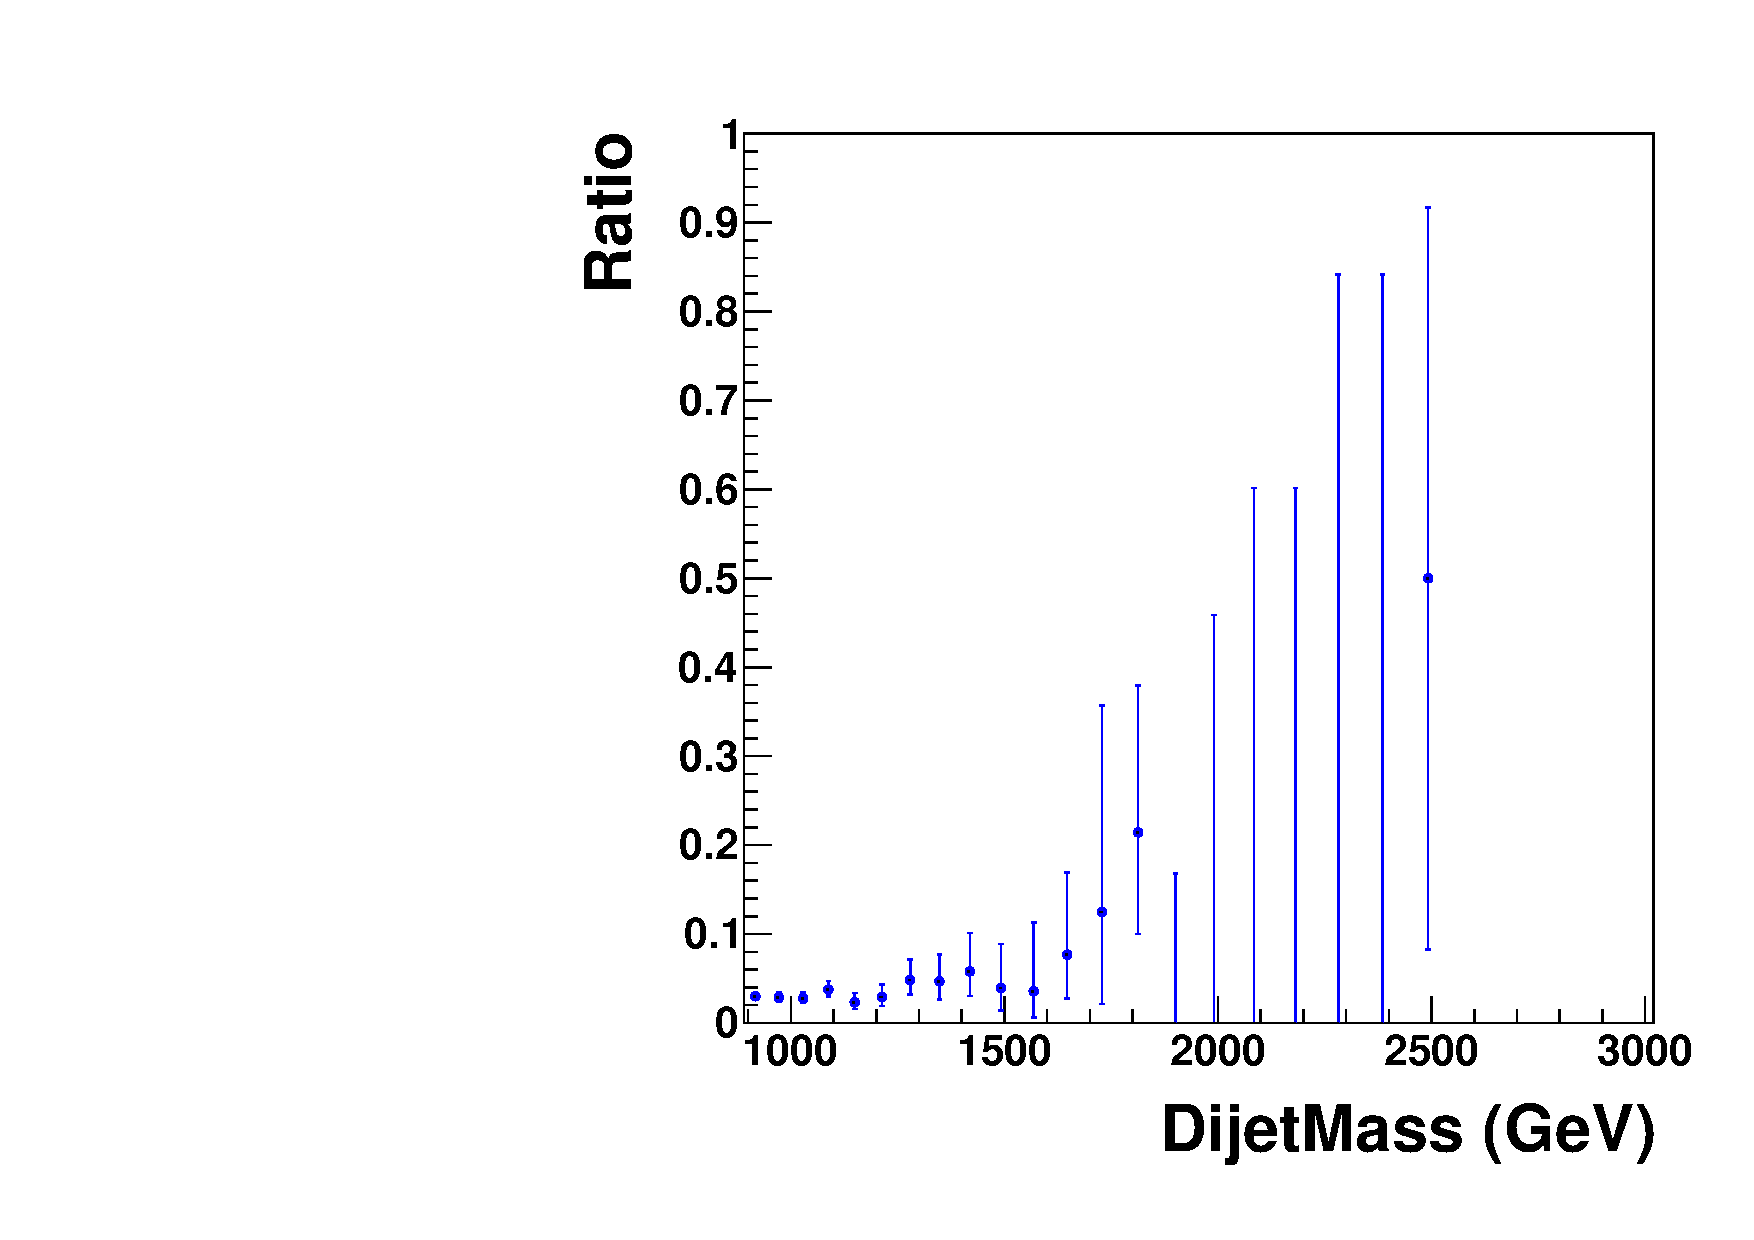
\includegraphics[width=0.49\textwidth, height=0.45\textwidth]{HqqqqZqqfigs/HbbHww/LowHPurityRatio.pdf}
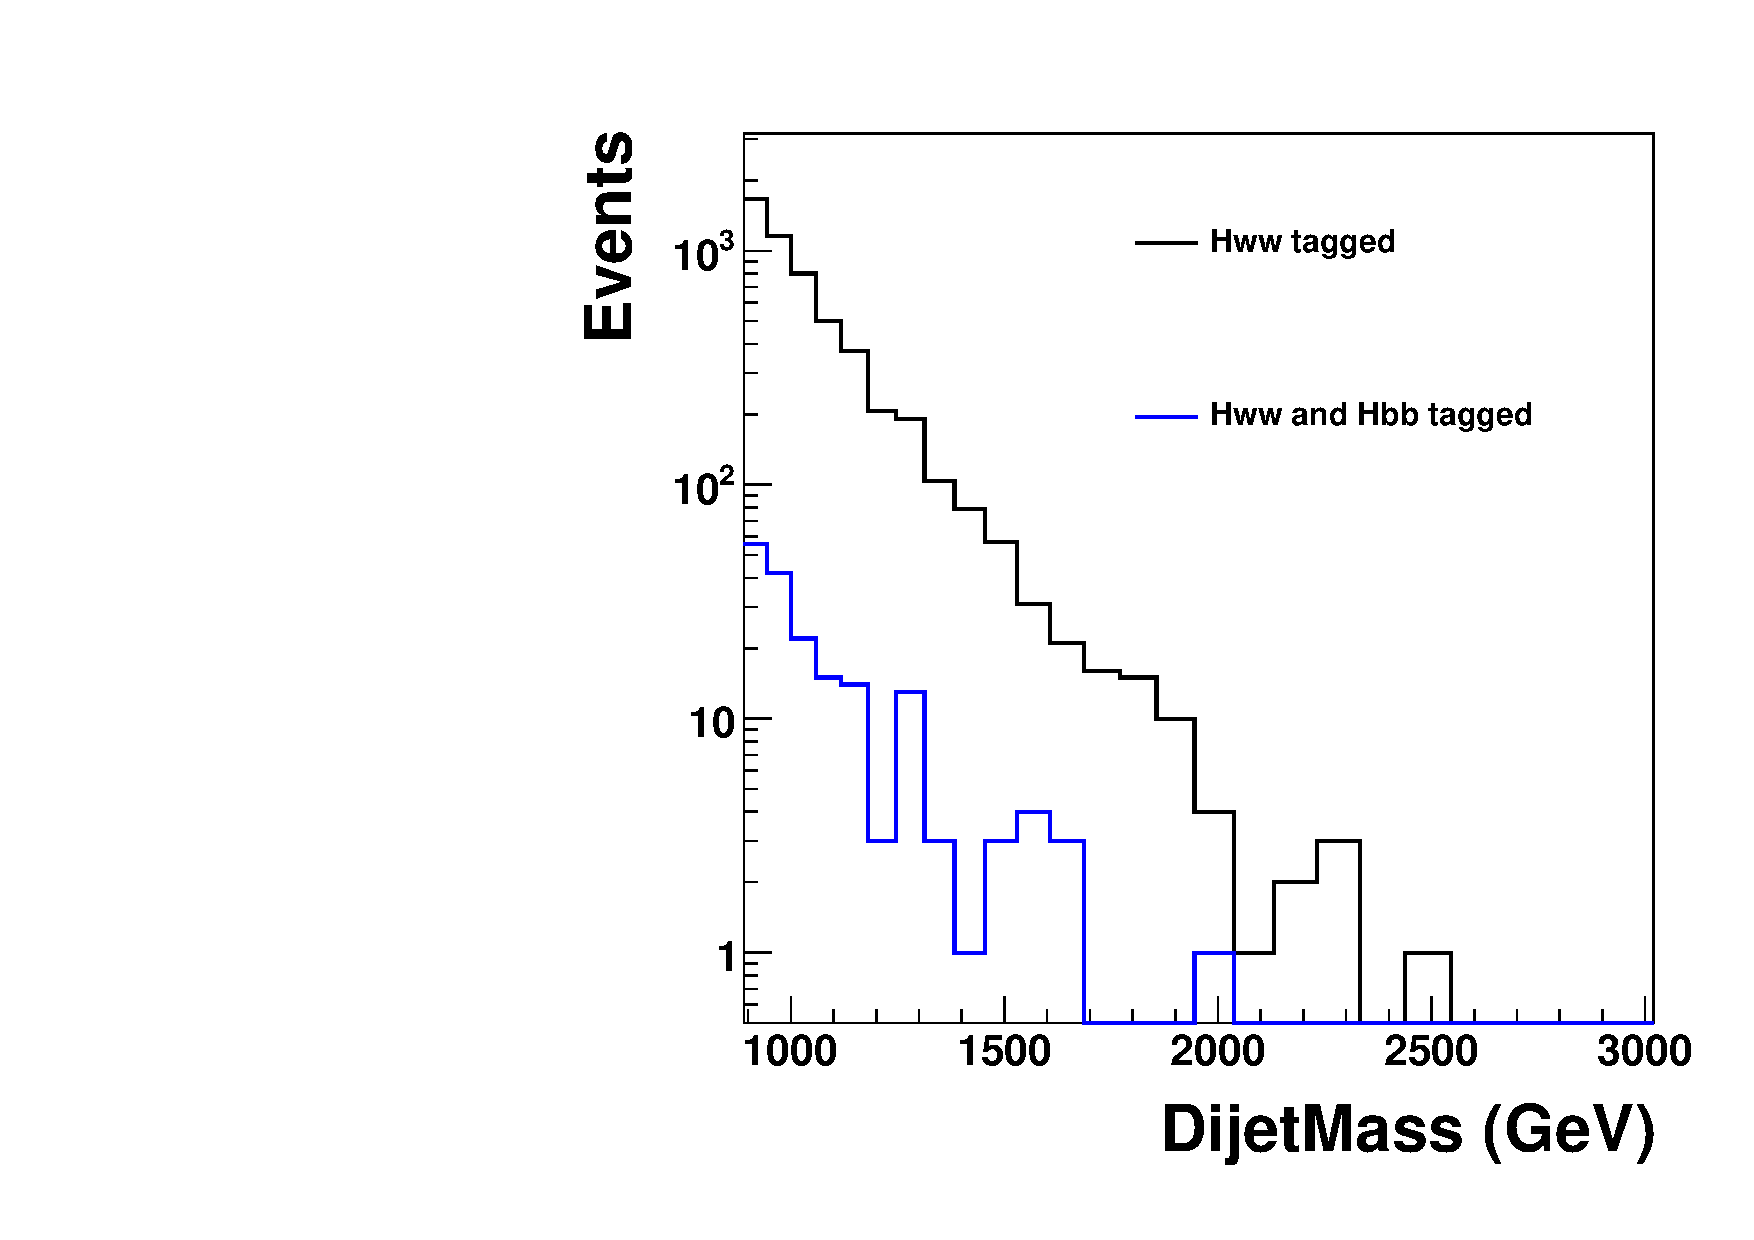
\includegraphics[width=0.49\textwidth, height=0.45\textwidth]{HqqqqZqqfigs/HbbHww/LowVPurity.pdf}
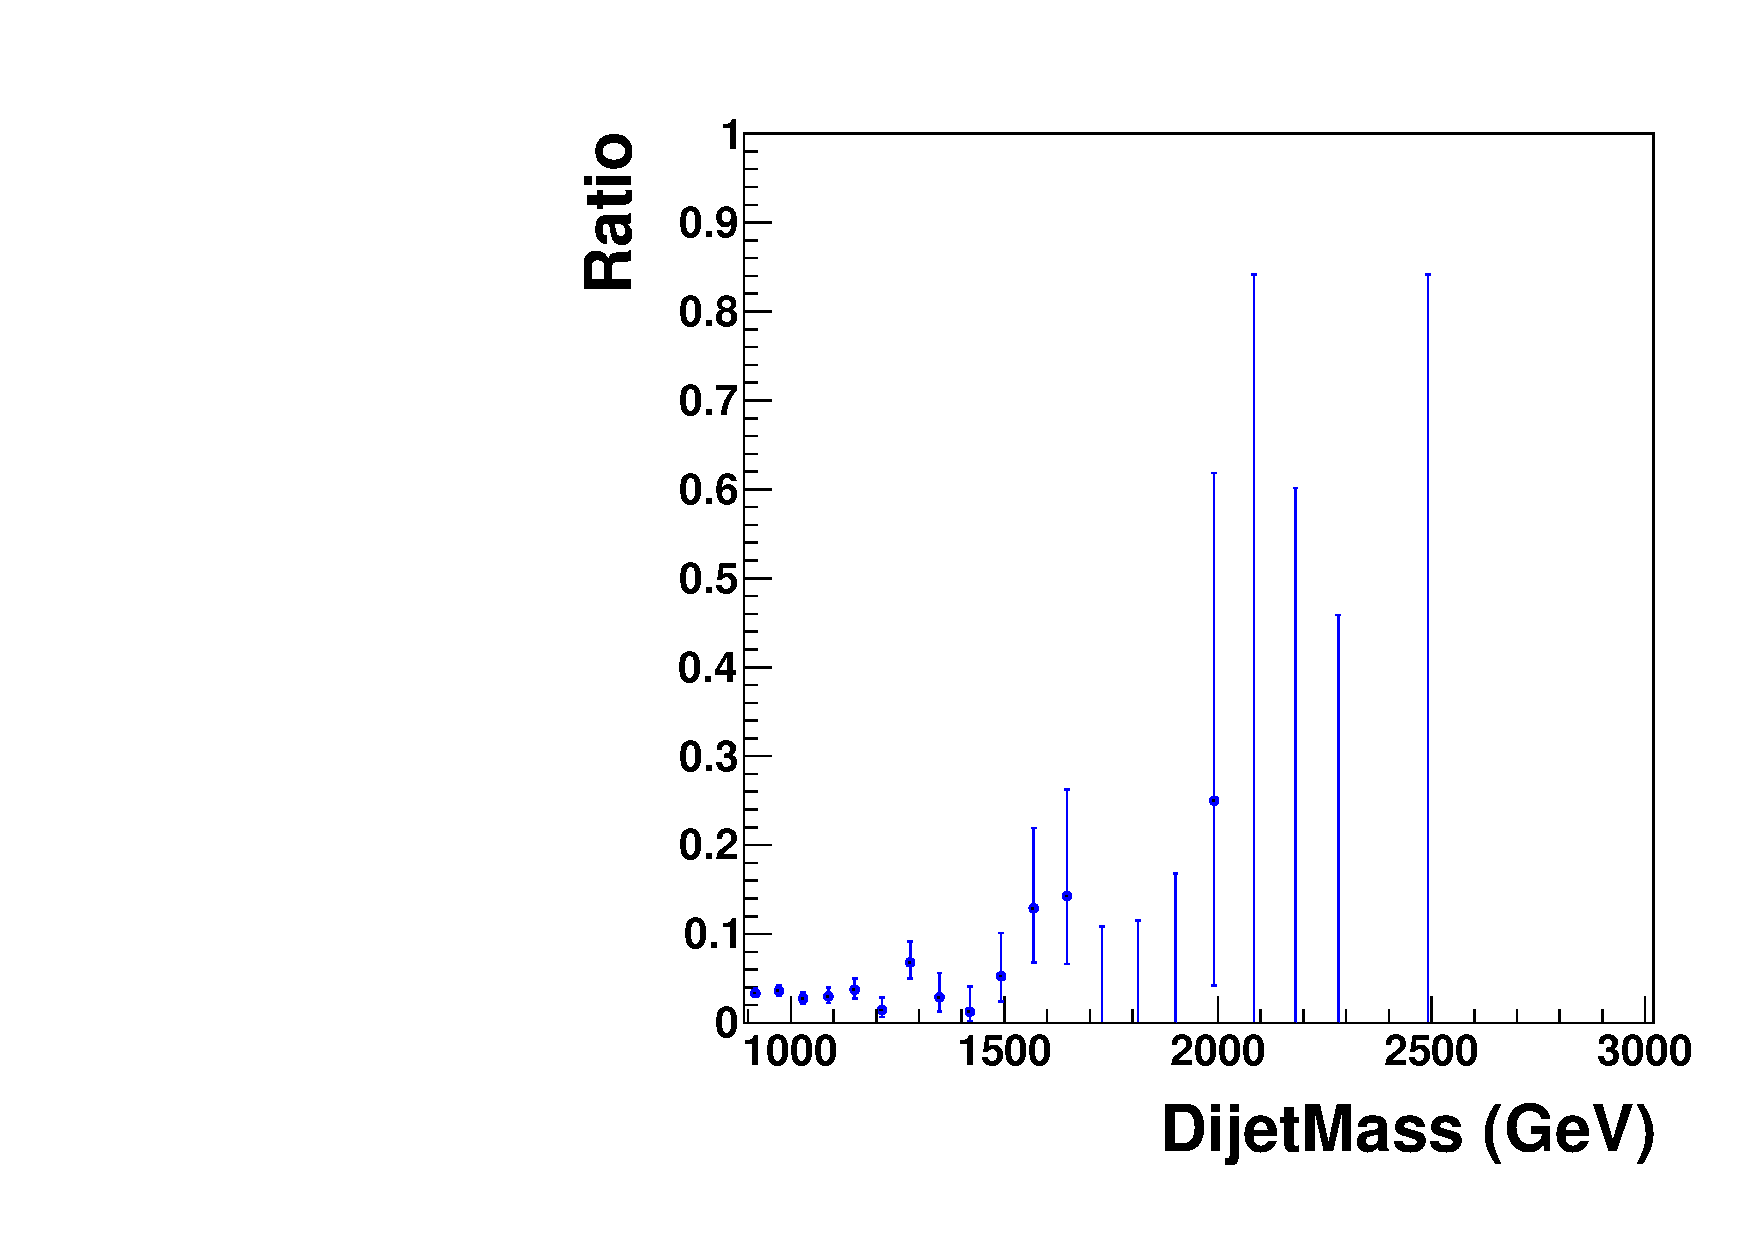
\includegraphics[width=0.49\textwidth, height=0.45\textwidth]{HqqqqZqqfigs/HbbHww/LowVPurityRatio.pdf}
\end{center}
\caption{ 
  Left column: dijet mass distribution in data, for events passing the $\Hww$
  tagger (black), and for a subset of these events passing also 
  the $\Hbb$ tagger (blue).  Right column: the fraction of $\Hww$ tagged events
  also tagged by $\Hbb$.  Top row: the high purity $\Hww$ tagger 
  and high purity V-tagger.  
  Middle row : the low purity $\Hww$ tagger, high purity V tagger. 
  bottom row : the high purity $\Hww$ tagger, low purity V tagger. 
}
 % Middle row: the low purity $\Hww$ 
 % tagger. Bottom: the low purity V tagger.  
\label{fig:HbbRatio}
\end{figure}


\clearpage
